\documentclass[12pt, a4paper]{report}
\usepackage[top=1cm, left=1cm, right=1cm]{geometry}

\usepackage[utf8]{inputenc}
\usepackage[russian]{babel}

\usepackage{array}
\newcolumntype{M}[1]{>{\centering\arraybackslash}m{#1}}

\usepackage{graphicx}
\graphicspath{ {../plots/pictures/}{../circuit/}}
\usepackage{subcaption}
\usepackage{float}

\begin{document}
	\begin{titlepage}
		\begin{center}
			\vspace*{5cm}
			\Huge \textbf{ЭЛЕКТРОТЕХНИКА И ЭЛЕКТРОНИКА}

			\vspace{1cm}
			\Huge \textbf{Рабочая тетрадь}
			
			\vspace{5cm}
			\begin{flushright}
				\Large
				\begin{tabular}{>{\raggedleft\arraybackslash}p{5cm} p{8cm}}
					Преподаватель: & \hrulefill \\
					Факультет: & \hrulefill \\
					\large Студент: & \hrulefill \\
					\large Группа: & \hrulefill \\
					\large Вариант: & \hrulefill \\
					\large Зачёт: & \hrulefill \\
					\large "\rule{1cm}{0.5pt}" & \rule{5cm}{0.5pt} 2024г. \\
				\end{tabular}
			\end{flushright}

			\vspace*{\fill}
			\Large Москва 2024
		\end{center}
	\end{titlepage}
	
	\pagenumbering{arabic}

	\begin{center}
		Лабораторная работа №1
		
		\large ЛИНЕЙНАЯ ЭЛЕКТРИЧЕСКАЯ ЦЕПЬ ПОСТОЯННОГО ТОКА	

		\textbf{Цель работы}
	\end{center}
	\par Исследование цепи постоянного тока.

	\begin{center}
		\textbf{Задачи}
	\end{center}
	\begin{enumerate}
		\item Рассчитать цепь при заданных параметрах.
		\item Исследовать цепь при изменении сопротивления нагрузки.
		\item Сравнить результаты расчета и исследования цепи.
		\item Записать выводы по результатам.
	\end{enumerate}

	\begin{center}
		\textbf{Ход работы}	
	\end{center}	
	\begin{enumerate}
		\item Рассчитать цепь (Рис. \ref{circuit}).	
			\begin{figure}[h]
				\centering
				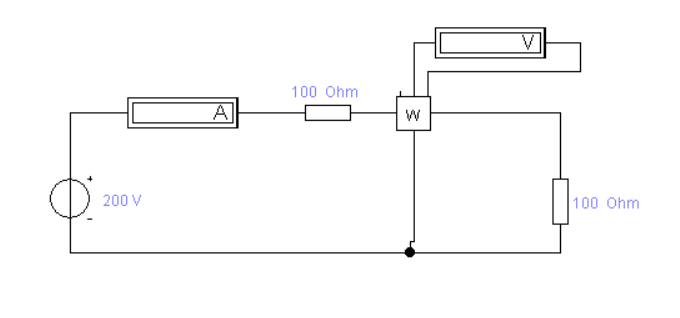
\includegraphics[width=1\textwidth]{circuit.png}
				\caption{Рассчетная цепь.}
				\label{circuit}
			\end{figure}
		\item Заполнить таблицу.	
			\newline
			\begin{tabular}{||M{4cm} | M{1.5cm} | M{1.5cm} | M{1.5cm} | M{1.5cm} | M{1.5cm} | M{1.5cm}||}
				\hline 
				Параметры цепи & \( R_{load} = 0 \) & \( R_{load} = R_{line} = 100 Ом \) & \( R_{load} = R + 100 Ом \) & \( R_{load} = R + 300 Ом \) & \( R_{load} = R + 500 Ом \) & \( R_{load} = R = 700 Ом \) \\

				\hline
				Ток, I, А & 2 & 1 & 0.5405 & 0.3509 & 0.2597 & 0.2062 \\

				\hline 
				Мощность источника, \newline \( P_{source} = E*I, \) Вт & 400 & 200 & 108.1 & 70.18 & 51.94 & 41.24 \\

				\hline
				Мощность нагрузки, \newline \( P_{load} = I^2*R, \) Вт & 0 & 100 & 78.88 & 57.87 & 45.19 & 36.99 \\

				\hline
				К.П.Д. цепи, \newline \( \eta = \frac{P_{load}}{P_{source}}*100\% \), \% & 0 & 50 & 73 & 82 & 87 & 90 \\
				\hline
			\end{tabular}
		\item Построить зависимости от \(R_{load}\) (Рис. \ref{plots}).
			\newline
			\begin{figure}[H]
				\begin{subfigure}{0.5\linewidth}
					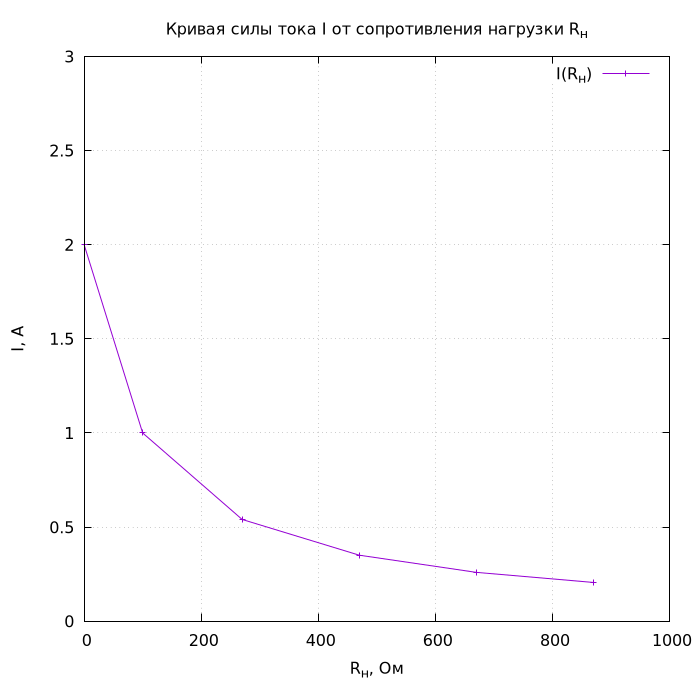
\includegraphics[width=\linewidth]{I_R.png}
				\end{subfigure}
				\hfill
				\begin{subfigure}{0.5\linewidth}
					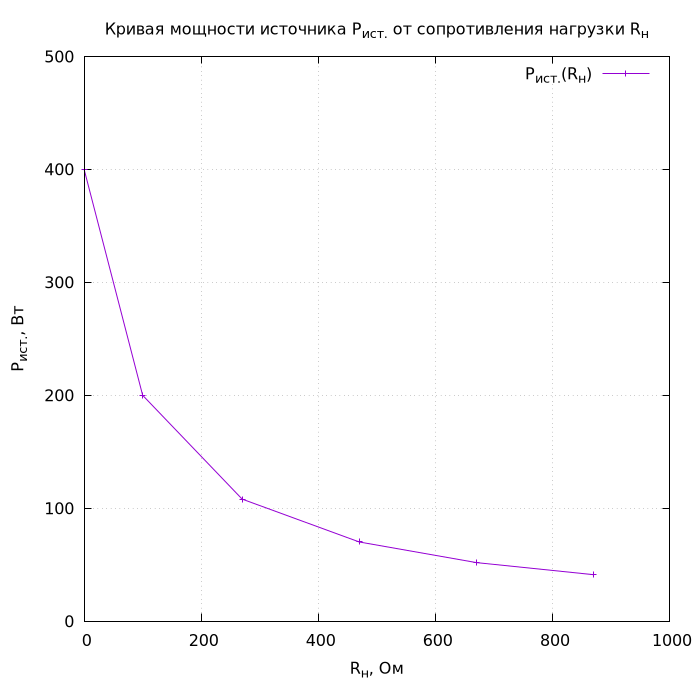
\includegraphics[width=\linewidth]{P_ist_R.png}
				\end{subfigure}
				\medskip
				\begin{subfigure}{0.5\linewidth}
					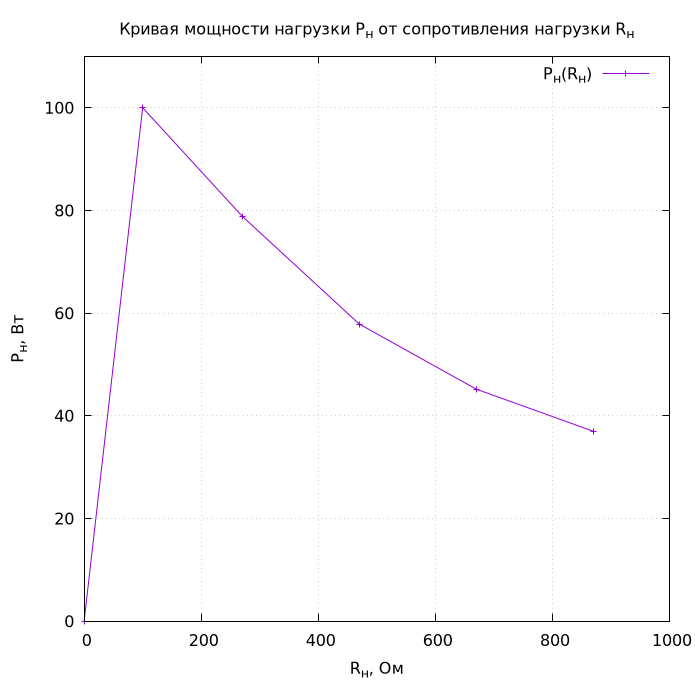
\includegraphics[width=\linewidth]{P_n_R.png}
				\end{subfigure}
				\begin{subfigure}{0.5\linewidth}
					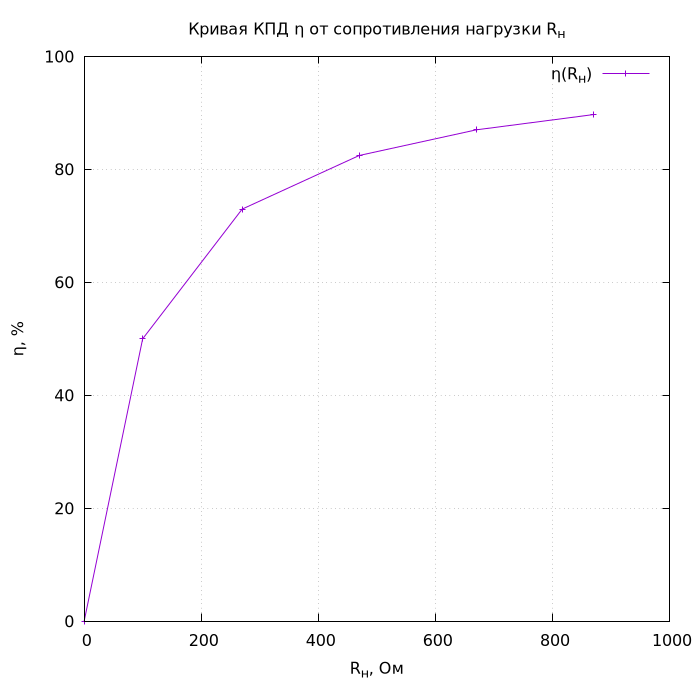
\includegraphics[width=\linewidth]{n_R.png}
				\end{subfigure}

				\caption{Графики.}
				\label{plots}
			\end{figure}
	\end{enumerate}

	\begin{center}
		\textbf{Выводы}
	\end{center}
	\par В ходе лабораторной работы я исследовал цепь постоянного тока. При изменении сопротивления нагрузки ток в цепи изменяется в обратной зависимости. Мощность, выделяемая на источнике, также уменьшается с увеличением сопротивления нагрузки. Мощность, протекающая через нагрузку, постепенно увеличивается с ростом сопротивления, достигая наибольшего значения и затем уменьшаясь. К.П.Д. цепи возрастает вместе с увеличением сопротивления нагрузки.
	\par Проделанная работа показанывает, что с увеличением сопротивления нагрузки полезная мощность возрастает, и К.П.Д. также имеет тенденцию к увеличению. Это связано с тем, что при низком сопротивлении нагрузки большая часть мощности идет на потери в виде тепла, в то время как при большем сопротивлении нагрузка более эффективно использует подводимую мощность.
\end{document}


